\documentclass{tufte-handout}

\title{Assignment-4: Memory Hierarchy: Cache}
  
  \author[]{Arnab Das, u1014840}
  
  %\date{28 March 2010} % without \date command, current date is supplied
  
  %\geometry{showframe} % display margins for debugging page layout
  
  % preamble.tex

\usepackage{graphicx} % allow embedded images
    \setkeys{Gin}{width=\linewidth,totalheight=\textheight,keepaspectratio}
    \graphicspath{{graphics/}} % set of paths to search for images
  \usepackage{tikz}
  \usetikzlibrary{shapes.geometric, arrows}
  \usepackage{amsmath}  % extended mathematics
  \usepackage{booktabs} % book-quality tables
  \usepackage{units}    % non-stacked fractions and better unit spacing
  \usepackage{multicol} % multiple column layout facilities
  \usepackage{lipsum}   % filler text
  \usepackage{fancyvrb} % extended verbatim environments
    \fvset{fontsize=\normalsize}% default font size for fancy-verbatim environments
  \usepackage{amsthm}
  \usepackage{thmtools}
  \usepackage{amssymb}
  %\usepackage[table]{xcolor}
  \usepackage{color}

  \newcommand*{\QEDA}{\hfill\ensuremath{\blacksquare}}%

  \newcommand{\stall}{\textcolor{red}{Stall}}
  %\newcommand{\cellstall}{\cellcolor{red}\textcolor{white}{\textbf{Stall}}}

  % Standardize command font styles and environments
  \newcommand{\doccmd}[1]{\texttt{\textbackslash#1}}% command name -- adds backslash automatically
  \newcommand{\docopt}[1]{\ensuremath{\langle}\textrm{\textit{#1}}\ensuremath{\rangle}}% optional command argument
  \newcommand{\docarg}[1]{\textrm{\textit{#1}}}% (required) command argument
  \newcommand{\docenv}[1]{\textsf{#1}}% environment name
  \newcommand{\docpkg}[1]{\texttt{#1}}% package name
  \newcommand{\doccls}[1]{\texttt{#1}}% document class name
  \newcommand{\docclsopt}[1]{\texttt{#1}}% document class option name
  \newenvironment{docspec}{\begin{quote}\noindent}{\end{quote}}% command specification environment
  \declaretheorem[thmbox=S]{theorem}
  \declaretheoremstyle[
spaceabove=6pt, spacebelow=6pt,
headfont=\normalfont\bfseries,
notefont=\mdseries, notebraces={(}{)},
bodyfont=\normalfont,
postheadspace=1em,
qed=\qedsymbol
]{mystyle}
\declaretheorem[style=mystyle,numbered=no]{Proof}
\declaretheorem[thmbox=S]{example}
\declaretheorem[thmbox=S]{Definition}

  
  \begin{document}
  
  \maketitle% this prints the handout title, author, and date
  

 \setcounter{secnumdepth}{1}

\newpage

\section{$\textbf{Cache Hierarchy}$}
	All the 2000 load instructions will access L1-cache to check for a hit. Since the tag and data access in L1 is parallel, hence the lookup for all 2000 instructions is 1 cycle each(equqal to the tag access time). Hence, the time spent in the lookup for the L1 cache is
	\[
		L1_t = 2000\ cycles
	\]

	Given the L1-cache hit rate is $50\%$,  hence number of instructions$( say\ n_2)$ that get forwarded to the L2 cache is 1000. All $n_2$ instructions will be required to access the tag, but only the hits gets to access data. Thus the time spent in the L2 cache lookup and data access is
	\begin{eqnarray*}
		L2_t &=& n_2\times 3 + (55\%\ of\ n_2)\times 18 \\
		L2_t &=& 1000\times 3 + (55\%\ of\ 100)\times 18 = 3000 + 550\times 18 = 3000 + 9900 = 12900\ cycles \\
	\end{eqnarray*}

	Given the hit rate of L2 cache is 55\%, hence number of instructions($n_3$) that get forwarded to the L3 cache is 450. Given the hit rate of L3 is 75\%, then the time spent in L3 cache lookup and data access is
	\begin{eqnarray*}
		L3_t &=& n_3\times 25 + (75\% of\ n_3)\times 85 \\ 
		L3_t &=& 450\times 25 + (75\% of\ 450)\times 85 = 11250 + 28687.5 = 39937.5\ cycles \\ 
	\end{eqnarray*}

	Given the hit rate of L3 cache is 75\%, hence of instructions($n_M$) that gets forwarded to Main memory is 112.5. Then time spent in Main Memory access will be
	\[
		MM_t = n_M\times 400 = 112.5 \times 440 = 49500	
	\]

	Thus, total number of cycles required to complete all 2000 load instructions is
	\[
		Total\ Time\ = L1_t + L2_t + L3_t + MM_t = 2000 + 12900 + 39937.5 + 49500 = 104337.5\ cycles
	\]

\section{$\textbf{Performance Metric}$}
	\begin{eqnarray*}
		Hit\ time,\ t_h &=& 5\ cycles \\
		Miss\ Penalty,\ t_m &=& 150\ cycles \\
		Miss\ Rate,\ r_m &=& = 0.2 \\
		AMAT &=& t_h + r_mt_m = 5 + 0.2\times 150 = 35 \\
	\end{eqnarray*}

\section{$\textbf{Cache Addressing}$}
	Given the Main Memory is 8GB, hence the required number of bits required for this address space is 33 bits.
	\subsection{$\textbf{L1 cache}$}
		\begin{eqnarray*}
			\mbox{Cache Size} &=& 32KB     \\
			\mbox{Block Size} &=& 16B = 2^4 B      \\
			\mbox{hence, Offset bits} &=& 4     \\
			\mbox{Number of Blocks} &=& \dfrac{Cache\ size}{Block\ Size} = \dfrac{32KB}{16B} = \dfrac{2^5 \times 2^{10}}{2^4} = 2^{11}      \\
			\mbox{hence, index bits} &=&  11    \\
			\mbox{hence, Tag bits} &=& 33 -4 -11 = 18      \\
			\mbox{Tag Array Size} &=& 2^{11}\times 18 bits = 2^{8}\times 18 B = 4.5 KB\\
			\mbox{Data Array Size} &=& \mbox{Same as the cache size} = 32KB \\
			\mbox{Total Size} &=& 32 KB + 4.5 KB = 36.5 KB\\
		\end{eqnarray*}

	\subsection{$\textbf{L2 cache}$}
		\begin{eqnarray*}
			\mbox{number of ways} &=& 4   \\
			\mbox{Each cache line size} &=& 64B = 2^6 B  \\
			\mbox{hence, Offset bits} &=& 6 \\
			\mbox{Block size} &=& 4\times 64B = 256 B  = 2^8 B \\
			\mbox{Cache Size} &=& 1MB = 2^{20}B   \\
			\mbox{Number of Blocks} &=& \dfrac{Cache\ Size}{Block\ Size}   = \dfrac{2^{20}}{2^8} = 2^{12}\\
			\mbox{hence, index bits} &=& 12  \\
			\mbox{hence, Tag bits} &=& 33 - 6 - 12 = 15  \\
			\mbox{Tag Array Size} &=& 4 \times 2^{12} \times 15 bits= 2^{11} \times 15 B = 30 KB\\
			\mbox{Data Array Size} &=& \mbox{Same as cache size} = 1MB \\
			\mbox{Total Size} &=& 30KB + 1MB \\
		\end{eqnarray*}

\section{$\textbf{Cache Replacement Policies}$}
	\subsection{Program-1}
	The following figures details the application of the ideal, LRU and MRU replacement policies to program-1.
	\begin{figure}[h!]
	\label{fig:p1ideal}
	\centering
	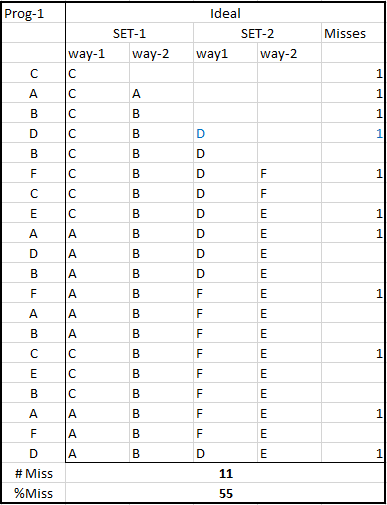
\includegraphics[width = 6in, height = 6in]{p1ideal}
	\caption{Program-1 Ideal replacement}
	\end{figure}
	
	\begin{figure}[h!]
	\label{fig:p1lru}
	\centering
	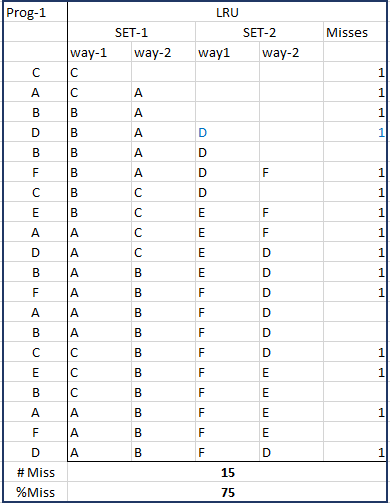
\includegraphics[width = 6in, height = 6in]{p1lru}
	\caption{Program-1 LRU replacement}
	\end{figure}
	
	\begin{figure}[h!]
	\label{fig:p1mru}
	\centering
	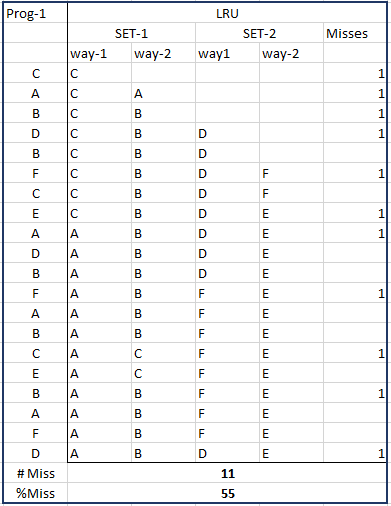
\includegraphics[width = 6in, height = 6in]{p1mru}
	\caption{Program-1 MRU replacement}
	\end{figure}

	To summarize, the miss rates for program-1 will be
	\begin{eqnarray*}
		Ideal &=& 55\% \\
		LRU &=& 75\% \\
		MRU &=& 55\% \\
	\end{eqnarray*}

\newpage
\newpage
	\subsection{Program-2}
	The following figures details the application of the ideal, LRU and MRU replacement policies to program-2.
	\begin{figure}[h!]
	\label{fig:p2ideal}
	\centering
	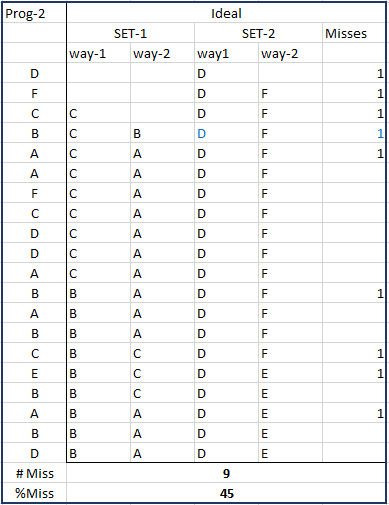
\includegraphics[width = 6in, height = 6in]{p2ideal}
	\caption{Program-2 Ideal replacement}
	\end{figure}

	\begin{figure}[h!]
	\label{fig:p2lru}
	\centering
	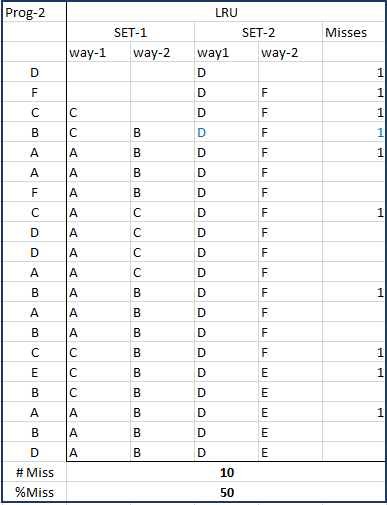
\includegraphics[width = 6in, height = 6in]{p2lru}
	\caption{Program-2 LRU replacement}
	\end{figure}

	
	\begin{figure}[h!]
	\label{fig:p2mru}
	\centering
	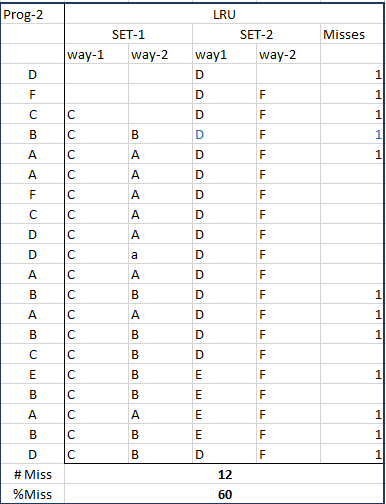
\includegraphics[width = 6in, height = 6in]{p2mru}
	\caption{Program-2 MRU replacement}
	\end{figure}

	To summarize, the miss rates for program-2 will be
	\begin{eqnarray*}
		Ideal &=& 45\% \\
		LRU &=& 50\% \\
		MRU &=& 60\% \\
	\end{eqnarray*}




		
  \bibliography{cs6810}
  \bibliographystyle{plainnat}
  
  \end{document}
